\documentclass[11pt]{article}
\usepackage{fontspec}
\setmainfont{DejaVu Serif}[Scale=0.93]
\setsansfont{DejaVu Sans}[Scale=0.93]
\setmonofont{DejaVu Sans Mono}[Scale=0.82]
\usepackage{amssymb}
\usepackage[a4paper,margin=2.2cm]{geometry}
\usepackage{xcolor}
\usepackage{titlesec}
\usepackage{enumitem}
\usepackage{booktabs}
\usepackage{tabularx}
\usepackage{array}
\usepackage{tikz}
\usetikzlibrary{positioning}

\definecolor{navy}{RGB}{19,40,82}
\definecolor{rulegrey}{RGB}{180,190,205}
\definecolor{accent}{RGB}{0,110,90}
\emergencystretch=3em
\hbadness=10000
\renewcommand{\arraystretch}{1.15}
\newcolumntype{R}{>{\raggedright\arraybackslash}X}
\newcommand{\pcol}[1]{>{\raggedright\arraybackslash}p{#1}}

\titleformat{\section}{\Large\bfseries\sffamily\color{navy}}{}{0pt}{}
\titleformat{\subsection}{\large\bfseries\sffamily\color{navy}}{}{0pt}{}
\titleformat{\subsubsection}{\normalsize\bfseries\sffamily\color{navy}}{}{0pt}{}
\titlespacing*{\section}{0pt}{1.2em}{0.4em}
\titlespacing*{\subsection}{0pt}{0.8em}{0.2em}
\titlespacing*{\subsubsection}{0pt}{0.6em}{0.15em}
\setlength{\parindent}{0pt}
\setlength{\parskip}{0.5em}
\setlist[itemize]{leftmargin=1.3em,itemsep=0.12em,topsep=0.2em}
\setlist[enumerate]{leftmargin=1.5em,itemsep=0.12em,topsep=0.2em}
\newcommand{\ra}{$\rightarrow$}
\newcommand{\key}[1]{\textbf{\color{navy}#1}}
\newcommand{\tc}[1]{\texttt{\small #1}}

\begin{document}

{\sffamily\bfseries\color{navy}\LARGE Część 2 --- Tor mocy (drugi schemat) i pełna specyfikacja Stateflow}\\[3pt]
{\sffamily\large\color{navy} Złoty wzorzec EVSE w architekturze 3 pętli + emulator auta}\\[5pt]
{\color{rulegrey}\rule{\linewidth}{1pt}}\\[3pt]
{\sffamily\small Dawid Cekała \quad$\cdot$\quad projekt AMPERE POINT \quad$\cdot$\quad wersja 1 \quad$\cdot$\quad 16 czerwca 2026}

\vspace{0.5em}

Dokument realizuje dwa punkty planu v4: \key{drugi schemat} (tor mocy) oraz \key{pełną specyfikację Stateflow} (obie karty, z architekturą 3 pętli). Honoruje korekty z addendów: \key{Stateflow = aktorzy} (odgrywają zachowanie wg normy), \key{komparator = sędzia} (klasyfikuje); przez granicę auto↔ładowarka idzie \key{tylko napięcie CP} (i PWM z powrotem) --- reszta sygnałów jest wewnętrzna danej strony.

% ============================================================
\section{1. Tor mocy --- drugi schemat}

\key{Po co osobny schemat:} dwa z trzech kluczowych scenariuszy nie mają gdzie zaistnieć na schemacie sygnałowym CP --- \key{weryfikacja licznika kWh} (całka mocy po czasie) i \key{DLB} (suma prądów vs bezpiecznik) żyją w torze mocy. To obwód \key{niełączący się elektrycznie} ze schematem CP; spina je \key{tylko} sygnał \tc{contactor\_cmd} (z wetem bezpieczeństwa).

\begin{center}
\resizebox{0.96\linewidth}{!}{%
\begin{tikzpicture}[font=\sffamily\footnotesize,
 b/.style={draw=navy,thick,rounded corners,fill=navy!7,align=center,inner sep=5pt,minimum height=1.05cm,text width=2.5cm},
 g/.style={draw=accent,thick,rounded corners,fill=accent!8,align=center,inner sep=5pt,text width=4.6cm}]
 \node[b](src){Sieć AC\\L / N / PE\\230 / 400 V};
 \node[b,right=1.0cm of src](k){Stycznik\\(K)};
 \node[b,right=1.0cm of k](m){Licznik\\energii (kWh)};
 \node[b,right=1.0cm of m](load){Obciążenie\\= ład. pokładowa\\auta ($I_{charge}$)};
 \draw[->,very thick](src)--(k);
 \draw[->,very thick](k)--(m);
 \draw[->,very thick](m)--(load);
 \node[g,below=1.25cm of k](gate){\textbf{Bramka stycznika}\\\tc{close = contactor\_cmd} \textbf{AND} \tc{not(fault)}};
 \draw[->,very thick,accent](gate)--(k);
 \node[align=left,font=\scriptsize,below=0.15cm of gate,text width=8cm]
   {\tc{contactor\_cmd} $\leftarrow$ \textbf{pętla 2} (sterowanie: zamknij w normalnej pracy)\\
    \tc{fault} $\leftarrow$ \textbf{pętla 1} (bezpieczeństwo: nadrzędne weto / odcięcie)};
\end{tikzpicture}}
\end{center}

Schemat jednokreskowy (tor 1- lub 3-fazowy). \key{Elementy i role:}

\begin{center}
\begin{tabularx}{\linewidth}{@{}\pcol{5.6cm} R@{}}
\toprule
\textbf{Element (Simscape)} & \textbf{Rola} \\
\midrule
\tc{AC Voltage Source} (230/400 V) & sieć zasilająca tor mocy \\
\tc{Ideal Switch} (stycznik K) & przełącza przepływ energii; sterowany bramką \tc{close} \\
Blok licznika: \tc{Current Sensor} + \tc{Voltage Sensor} + \tc{Product} ($P{=}UI$) + \tc{Integrator} + \tc{Gain} $1/3600$ & liczy energię (kWh); model „raportowanej'' kWh z konfigurowalnym błędem (offset / dryf / kwantyzacja) \\
\tc{Controlled Current Source} (obciążenie) & udaje ład. pokładową auta pobierającą \tc{i\_demand} (do \tc{I\_offer}) \\
\tc{Logical Operator} (AND, NOT) & bramka: \tc{close = contactor\_cmd AND not(fault)} \\
\tc{Solver Configuration} + \tc{Electrical Reference} & obowiązkowe dla obwodu Simscape \\
\bottomrule
\end{tabularx}
\end{center}

\key{Logika stycznika (sedno).} Stycznik jest jeden; władza nad nim \key{asymetryczna}:
\begin{itemize}
  \item \key{Pętla 2} (sterowanie) załącza/wyłącza w \key{normalnej} pracy: B\ra{}C OK \ra{} \tc{contactor\_cmd=1}; koniec sesji / odpięcie \ra{} \tc{=0}.
  \item \key{Pętla 1} (bezpieczeństwo) ma \key{nadrzędne weto}: rozwiera stycznik niezależnie od pętli 2 (RCD, stan E/F, sklejony styk, nadprąd). W realu zwykle sprzętowo przerywa obwód cewki.
\end{itemize}
\[ \texttt{stycznik\_zamknięty} = (\texttt{pętla2 każe zamknąć}) \;\wedge\; \neg(\texttt{usterka pętli1}) \]
\key{Diagnostyka (dla komparatora):} stycznik nie otwiera na usterkę \ra{} defekt \key{pętli 1}; złe duty/prąd przy zamkniętym styczniku \ra{} \key{pętla 2}; przekłamane kWh \ra{} \key{pętla 3}.

% ============================================================
\section{2. Pełny Stateflow --- przegląd i interfejs}

\key{Dwie karty Stateflow = dwaj aktorzy:} „Emulator auta'' i „Złoty wzorzec EVSE''. \key{Nie rozmawiają wprost} --- wymieniają się \key{tylko przez fizyczny węzeł CP} (Simscape jako „kabel''). To czyni model cyfrowym bliźniakiem, nie samym diagramem logiki.

\key{Pętla obiegu sygnału:}
\tc{Emulator auta} ustawia \tc{StateC}/\tc{veh\_cmd} \ra{} mostek \ra{} switch/R w Simscape \ra{} \key{napięcie CP się ustala} \ra{} \tc{Voltage Sensor} \ra{} mostek \ra{} \tc{cp\_voltage} \ra{} \tc{Złoty wzorzec} decyduje \tc{duty}/\tc{contactor\_cmd} \ra{} mostek \ra{} źródło PWM + stycznik \ra{} koło się zamyka.

\begin{center}
\begin{tabularx}{\linewidth}{@{}\pcol{2.7cm}\pcol{2.7cm} R@{}}
\toprule
\textbf{Sygnał} & \textbf{Kierunek} & \textbf{Znaczenie} \\
\midrule
\tc{cp\_voltage} & CP \ra{} wzorzec & napięcie linii CP (jedyne, co realnie przekracza granicę) \\
\tc{duty} & wzorzec \ra{} CP & wypełnienie PWM (koduje \tc{I\_offer}=duty·0,6) \\
\tc{StateC}, \tc{veh\_cmd} & wewn. auta & które rezystory/diodę wpiąć (B/C, usterki) \\
\tc{i\_demand} & auto \ra{} tor mocy & prąd, jaki auto pobiera w stanie C \\
\tc{I\_offer} & wewn. wzorca & min(instalacja, kabel/PP, DLB, limit pętli 3) \\
\tc{contactor\_cmd} & wzorzec(p2) \ra{} moc & żądanie zamknięcia stycznika \\
\tc{fault\_p1} & wzorzec(p1) \ra{} bramka & weto bezpieczeństwa (otwiera stycznik) \\
\bottomrule
\end{tabularx}
\end{center}

% ============================================================
\section{3. Karta „Emulator auta'' (aktor: samochód)}

Pasywny elektrycznie --- tylko \key{wybiera rezystory/diodę} i (w stanie C) pobiera prąd. Prowadzony scenariuszem z sekwencera.

\begin{center}
\resizebox{0.96\linewidth}{!}{%
\begin{tikzpicture}[font=\sffamily\footnotesize,
 s/.style={draw=navy,thick,rounded corners,fill=navy!7,align=center,inner sep=5pt,text width=3.1cm,minimum height=1.25cm},
 f/.style={draw=accent,thick,rounded corners,fill=accent!8,align=center,inner sep=5pt,text width=3.0cm,minimum height=1.25cm}]
 \node[s](a){\textbf{A\_Unplugged}\\brak wpięcia\\\tc{i\_demand=0}};
 \node[s,right=2.0cm of a](b){\textbf{B\_Connected}\\dioda+R2 (9 V)\\\tc{StateC=0}};
 \node[s,right=2.0cm of b](c){\textbf{C\_Ready}\\+R3 (6 V), ładuje\\\tc{i\_demand}=min(\dots)};
 \node[f,below=1.0cm of b](flt){\textbf{Fault}\\usterka wstrzyknięta\\(brak diody / zwarcie CP)};
 \draw[->,thick](a)--(b) node[midway,above,font=\scriptsize]{cmd\_connect};
 \draw[->,thick](b)--(c) node[midway,above,font=\scriptsize]{cmd\_ready};
 \draw[->,thick](c) to[bend left=28] node[below,font=\scriptsize]{cmd\_stop} (b);
 \draw[->,thick](b) to[bend left=22] node[above,font=\scriptsize]{cmd\_unplug} (a);
 \draw[->,thick,accent](b)--(flt) node[midway,right,font=\scriptsize]{fault\_inject};
 \draw[->,thick,accent](flt) to[bend right=20] (a);
\end{tikzpicture}}
\end{center}

\begin{center}
\begin{tabularx}{\linewidth}{@{}\pcol{3.1cm} R@{}}
\toprule
\textbf{Stan} & \textbf{Akcje wejścia (entry) / wyjścia} \\
\midrule
\tc{A\_Unplugged} & \tc{veh\_cmd}: brak połączenia (wysoka impedancja); \tc{i\_demand=0}. CP $\approx$ +12 V. \\
\tc{B\_Connected} & wepnij \tc{diode}+\tc{R2}; \tc{StateC=0}; \tc{i\_demand=0}. CP $\approx$ 9 V. \\
\tc{C\_Ready} & \tc{StateC=1} (dołóż \tc{R3}); odczytaj duty z CP \ra{} \tc{i\_demand}=min(I\_offer, I\_car\_max). CP $\approx$ 6 V. \\
\tc{Fault} & zastosuj usterkę (\tc{no\_diode} / \tc{cp\_short} / złe PP); bodziec testowy. \\
\bottomrule
\end{tabularx}
\end{center}

% ============================================================
\section{4. Karta „Złoty wzorzec EVSE'' --- 3 zagnieżdżone pętle}

Wnętrze ładowarki (i wzorca) to trzy kaskadowe warstwy. Wyższa zadaje cele niższej; \key{pętla 1 zawsze może przebić wyższe w imię bezpieczeństwa}.

\begin{center}
\resizebox{0.95\linewidth}{!}{%
\begin{tikzpicture}[font=\sffamily\footnotesize,
 L/.style={draw=navy,thick,rounded corners,align=left,inner sep=6pt,text width=11cm,minimum height=1.0cm}]
 \node[L,fill=navy!4](l3){\textbf{Pętla 3 --- Aplikacja} (miękki real-time): Tuya/WiFi, RFID, OTA, \textbf{licznik kWh}, harmonogram, konfiguracja DLB, UI. Ustawia \emph{polityki/nastawy} (autoryzacja, limity prądu, okna czasowe). Nie dotyka stycznika.};
 \node[L,fill=navy!9,below=0.55cm of l3](l2){\textbf{Pętla 2 --- Sterowanie} (10 ms…s): FSM handshake A\ra B\ra C, decyzja \tc{duty} (= oferowany prąd), \textbf{DLB do 4 stacji}, \tc{contactor\_cmd}. „Mózg sterowania''.};
 \node[L,fill=navy!14,below=0.55cm of l2](l1){\textbf{Pętla 1 --- Odruch / Bezpieczeństwo} (ms, często sprzęt): front-end CP, zabezpieczenia (RCD typ A 30 mA, detekcja 6 mA DC, monitoring PE, sklejony styk, nadprąd). \emph{Weto}: usterka \ra{} stycznik otwarty natychmiast.};
 \draw[->,thick]([xshift=-3.2cm]l3.south)--([xshift=-3.2cm]l2.north) node[midway,left,font=\scriptsize]{nastawy};
 \draw[->,thick]([xshift=3.2cm]l2.north)--([xshift=3.2cm]l3.south) node[midway,right,font=\scriptsize]{raport};
 \draw[->,thick]([xshift=-3.2cm]l2.south)--([xshift=-3.2cm]l1.north) node[midway,left,font=\scriptsize]{żądania};
 \draw[->,thick]([xshift=3.2cm]l1.north)--([xshift=3.2cm]l2.south) node[midway,right,font=\scriptsize]{status};
 \node[draw=accent,thick,rounded corners,fill=accent!8,below=0.5cm of l1,text width=4cm,align=center,font=\scriptsize](sw){Stycznik (tor mocy)};
 \draw[->,thick,accent](l1.south)--(sw) node[midway,right,font=\scriptsize]{weto};
\end{tikzpicture}}
\end{center}

\subsection{4.1. Pętla 1 --- odruch / bezpieczeństwo}
Wejścia (w symulacji jako flagi wstrzykiwane): \tc{cp\_invalid} (CP w stanie E/F $\approx$ 0 V), \tc{rcd\_trip}, \tc{pe\_lost}, \tc{contactor\_welded}, \tc{overcurrent}. Wyjście: \key{\tc{fault\_p1}} (OR powyższych). Reakcja: \tc{fault\_p1=1} \ra{} \key{wymusza} otwarcie stycznika (nadpisuje pętlę 2). W Stateflow: stan \tc{Safe} \ra{} \tc{Tripped}; w \tc{Tripped} stycznik bezwarunkowo otwarty, powrót dopiero po skasowaniu usterki.

\subsection{4.2. Pętla 2 --- sterowanie (FSM handshake)}

\begin{center}
\resizebox{0.96\linewidth}{!}{%
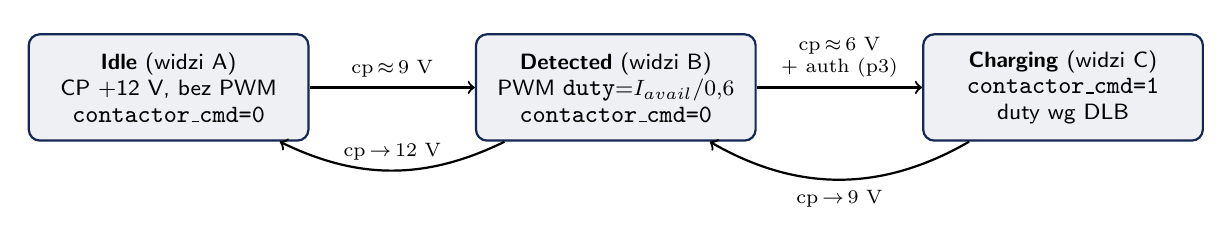
\begin{tikzpicture}[font=\sffamily\footnotesize,
 s/.style={draw=navy,thick,rounded corners,fill=navy!7,align=center,inner sep=5pt,text width=3.2cm,minimum height=1.35cm}]
 \node[s](idle){\textbf{Idle} (widzi A)\\CP +12 V, bez PWM\\\tc{contactor\_cmd=0}};
 \node[s,right=2.1cm of idle](det){\textbf{Detected} (widzi B)\\PWM \tc{duty}=$I_{avail}/0{,}6$\\\tc{contactor\_cmd=0}};
 \node[s,right=2.1cm of det](chg){\textbf{Charging} (widzi C)\\\tc{contactor\_cmd=1}\\duty wg DLB};
 \draw[->,thick](idle)--(det) node[midway,above,font=\scriptsize,align=center]{cp\,$\approx$\,9 V};
 \draw[->,thick](det)--(chg) node[midway,above,font=\scriptsize,align=center]{cp\,$\approx$\,6 V\\+ auth (p3)};
 \draw[->,thick](chg) to[bend left=30] node[below,font=\scriptsize]{cp\,$\to$\,9 V} (det);
 \draw[->,thick](det) to[bend left=26] node[above,font=\scriptsize]{cp\,$\to$\,12 V} (idle);
\end{tikzpicture}}
\end{center}

\begin{center}
\begin{tabularx}{\linewidth}{@{}\pcol{3.0cm}\pcol{3.8cm} R@{}}
\toprule
\textbf{Przejście} & \textbf{Warunek} & \textbf{Akcja} \\
\midrule
Idle \ra{} Detected & \tc{cp\_voltage} $\approx$ 9 V & włącz PWM, \tc{duty}=$I_{avail}/0{,}6$ \\
Detected \ra{} Charging & \tc{cp\_voltage} $\approx$ 6 V \textbf{i} \tc{auth\_ok} (p3) & \tc{contactor\_cmd=1} \\
Charging \ra{} Detected & \tc{cp\_voltage} $\to$ 9 V (stop) & \tc{contactor\_cmd=0} \\
$\ast$ \ra{} Idle & \tc{cp\_voltage} $\to$ 12 V (odpięto) & \tc{contactor\_cmd=0}, stop PWM \\
\bottomrule
\end{tabularx}
\end{center}

\key{Prąd oferowany:} \tc{I\_avail} = min(limit instalacji, obciążalność kabla z PP, limit DLB, limit pętli 3); \tc{duty} = \tc{I\_avail}/0,6 (10--85\%). \key{DLB:} gdy suma prądów zbliża się do bezpiecznika \ra{} obniż \tc{duty} (auto schodzi w kilka sekund); po odpięciu auta \ra{} dobierz wolną moc.

\subsection{4.3. Pętla 3 --- aplikacja}
Wejścia: \tc{rfid\_uid}, \tc{schedule}, \tc{dlb\_config}, \tc{user\_limit}. Wyjścia (nastawy dla pętli 2): \key{\tc{auth\_ok}} (autoryzacja), \tc{limit\_p3} (limit prądu / okno czasowe). Prowadzi też \key{licznik kWh} (niezerowalny) --- model raportowanej energii porównywany przez komparator z prawdziwą całką mocy.

\subsection{4.4. Bramka stycznika --- pseudokod}
\begin{quote}\ttfamily\small
fault\_p1 = cp\_invalid OR rcd\_trip OR pe\_lost OR welded OR overcurrent\\
contactor\_close = contactor\_cmd\_p2 AND (NOT fault\_p1)
\end{quote}
W Stateflow: pętla 1 \emph{wymusza} otwarcie (nadpisuje); pętla 2 tylko \emph{prosi} o zamknięcie. \emph{Otworzyć} może każda; otwarcie z pętli 1 wygrywa.

% ============================================================
\section{5. Mapowanie sim \ra{} HIL (most do sprzętu)}

To, co w symulacji jest blokiem-mostkiem, w sprzęcie staje się \key{peryferium MCU + układem pośredniczącym}. \key{Symulacja jest wprost specyfikacją adaptera.}

\begin{center}
\begin{tabularx}{\linewidth}{@{}\pcol{4.4cm}\pcol{2.9cm} R@{}}
\toprule
\textbf{Blok symulacji} & \textbf{Peryferium MCU} & \textbf{Układ elektryczny} \\
\midrule
PWM \ra{} Simulink-PS \ra{} Vsrc & timer / DAC & op-amp/komparator \ra{} $\pm$12 V (nadajnik CP) \\
Voltage Sensor \ra{} PS-Simulink & ADC + input-capture & dzielnik + clamp + offset (odbiór CP) \\
Switch/R3 (emulator auta) & GPIO & przekaźnik/MOSFET + dioda + bank R (PP) \\
\tc{contactor\_cmd} \ra{} Ideal Switch & GPIO + odczyt styku & driver cewki + styk pomocniczy \\
Licznik (Integrator) & SPI/UART / impuls & pomiar mocy (DUT) lub osobny miernik \\
\bottomrule
\end{tabularx}
\end{center}

\key{Dwa tryby (1:1):} \emph{Tryb symulacji} --- obie karty + „kabel'' Simscape; produkt = \key{katalog} par „bodziec \ra{} oczekiwana poprawna odpowiedź'' + tolerancja + pass/fail. \emph{Tryb HIL} --- „Emulator auta'' \ra{} adapter sprzętowy, „warstwa CP'' \ra{} realny kabel + ładowarka (DUT); \key{wzorzec + sekwencer + komparator + katalog zostają w software}. Prawdziwe usterki wychodzą \key{na sprzęcie}, nie w symulacji (wzorzec poprawny z definicji).

\end{document}
